\documentclass[a4paper]{cas-sc}
\usepackage[numbers,sort&compress]{natbib}
\usepackage{amsmath,amssymb,booktabs,tabularx,array,placeins,microtype}
\setlength{\emergencystretch}{2em}
\microtypesetup{protrusion=false}
\setlength{\textfloatsep}{20pt plus 3pt minus 2pt}
\setlength{\intextsep}{20pt plus 3pt minus 2pt}
\setlength{\floatsep}{18pt plus 3pt minus 2pt}
\makeatletter
\@fleqnfalse
\@mathmargin\@centering
\renewcommand\section{\@startsection{section}{1}{\z@}%
  {18pt plus 3pt minus 2pt}{9pt}%
  {\sectionfont\raggedright\hst[13pt]}}
\renewcommand\subsection{\@startsection{subsection}{2}{\z@}%
  {14pt plus 3pt minus 2pt}{6pt}%
  {\ssectionfont\raggedright}}
\renewcommand\subsubsection{\@startsection{subsubsection}{3}{\z@}%
  {12pt plus 2pt minus 2pt}{5pt}%
  {\sssectionfont\raggedright}}
\makeatother
\graphicspath{{figures/}}
\hypersetup{pdftitle={A spatial capillary correction for driven junction motion in double-obstacle multiphase-field simulations},pdfauthor={Ayas Alzanki},colorlinks=true,linkcolor=blue,citecolor=blue,urlcolor=blue}
\newcommand{\ph}{\boldsymbol{\phi}}
\newcommand{\RMS}{\mathrm{RMS}}
\newcommand{\HH}{d_{\mathrm H}}
\newcommand{\Dt}{\Delta t}
\ExplSyntaxOn
\cs_set:Npn \__first_footerline: { \small\sffamily A.~Alzanki }
\ExplSyntaxOff
\begin{document}
\shorttitle{Spatial capillary correction for driven junctions}
\shortauthors{A. Alzanki}
\title[mode=title]{A spatial capillary correction for driven junction motion in double-obstacle multiphase-field simulations}
\author[1]{Ayas Alzanki}[orcid=0009-0004-3121-3778]
\cormark[1]
\ead{azanki@kisr.edu.kw}
\affiliation[1]{organization={Energy and Building Research Center, Kuwait Institute for Scientific Research (KISR)},addressline={P.O. Box 24885},city={Safat},postcode={13109},country={Kuwait}}
\cortext[1]{Corresponding author.}
\begin{abstract}
Artificial interface thickness can produce substantial errors in the motion and shape of strongly driven multiphase junctions, even when binary-interface motion is accurately calibrated. We introduce a spatial capillary correction for compact-support double-obstacle models. A normalized ternary-product signal identifies junctions, and its maximum over a neighborhood sets a multiplier on the capillary contribution while leaving the bulk driving term unchanged. An optional component-memory rule suppresses selected sources after junction neighborhoods overlap. At matched width, grid and timestep, the correction reduces migration-speed error from 16.01\% to 0.45\% and aligned interface-shape RMS error from $0.1051W$ to $0.0060W$ in a driven unequal-energy benchmark. In a cold interacting-junction calculation, the whole correction reduces worst sampled Hausdorff errors from $0.1061W$ and $0.1408W$ to $0.02694W$ and $0.03058W$; local memory further reduces them to $0.01399W$ and $0.01814W$. Porting the fixed prescription to OpenPhase reduces migration-speed error from 25.53\% to 0.98\% and disappearance-time errors to approximately 1\%, although one late shape sample remains outside the chosen tolerance. The results establish a practical accuracy benefit in the tested driven-junction regimes and distinguish the simpler spatial correction from the additional, case-dependent benefit of interaction memory.
\end{abstract}
\begin{keywords}
Multiphase-field \sep Triple junction \sep Double-obstacle potential \sep Interface thickness \sep Numerical accuracy \sep Grain-boundary motion
\end{keywords}
\maketitle
\hypersetup{pdfauthor={Ayas Alzanki}}
\section{Introduction}
Phase-field simulation is widely used to study the formation and evolution of material microstructures \citep{moelans2008,tourret2022}. A grain or phase is represented by a continuous field that changes smoothly across an interface. The interface moves as the fields evolve, so its position need not be tracked explicitly. This description is useful when boundaries curve, meet or disappear during solidification, grain growth, coarsening and solid-state transformation. It also permits interface motion to be coupled to other processes: solidification models, for example, combine the phase fields with heat and solute transport \citep{boettinger2002}.

In a polycrystal, multiple fields distinguish the individual grains and allow their shapes, sizes and topology to evolve within one calculation \citep{krill2002}. Multiphase-field formulations accommodate different interfacial energies and mobilities for the boundaries between them \citep{steinbach1996,steinbach1999,steinbach2009}. These boundaries are connected through junctions. Their motion must therefore respect both interface kinetics and interfacial force balance, rather than reproduce the speed of an isolated planar boundary alone. Classical curvature-driven grain-boundary motion provides one sharp-interface reference \citep{mullins1956}; bulk driving forces introduce an additional contribution to interface motion. An error near a junction can consequently affect the shape and disappearance time of an entire neighboring grain.

Nanocrystalline materials provide context because their grain structures and stability change during thermal exposure. Studies of triple-junction drag show that finite junction mobility can affect grain-growth rates, size distributions and the transition from junction- to boundary-controlled growth \citep{johnson2014,miyoshi2026}. The direct numerical motivation here is strongly driven transformation-front motion: junction errors at practical diffuse widths can distort adjoining boundary shapes and grain-disappearance times \citep{hoffrogge2025}. Physical nanoscale junction drag is a distinct mechanism; the prescribed sharp-interface tests below neither calibrate that mobility nor validate a particular nanomaterial.

Computational interfaces are often widened to reduce simulation cost, so a quantitative method must reproduce intended motion at its chosen width as well as resolve its equations. Thin-interface analysis and corrections have been particularly successful for solidification \citep{karma1998,karma2001,eiken2006}; narrowing the region of latent-heat release or solute redistribution can further suppress anomalous interface effects there \citep{kim2004}. At multiphase junctions, several profiles and force channels coexist, and correct planar-front motion does not ensure correct junction motion. Benchmarks show sensitivity to interfacial-energy terms, mobility interpolation, resolution and bulk-force allocation \citep{daubner2023,nani2024,hoffrogge2025}. Speed, whole-boundary shape and event timing are therefore complementary measurements.

Several methods already address parts of this problem. Grose and Asimow \citep{grose2022} redistribute bulk driving forces among phase fields and combine this with profile correction and recursive transfer at junctions. Feyen and Moelans \citep{feyen2023} separate normal-profile restoration from physical curvature weighting in a high-driving-force model. Zhang et al. \citep{zhang2023large} extend the driving-force term to remain constant along interface normals in driven Allen--Cahn and concentration-coupled models, a different formulation from the local capillary modification tested here. Profile-informed finite-difference correction \citep{eiken2012}, isotropic spatial operators \citep{tang2024}, and hybrid nonlinear preconditioning for double-obstacle potentials \citep{sakane2026} reduce other important errors. Improved time integration can reduce the work needed to follow a trajectory \citep{seiz2026}, but does not by itself remove an inaccurate finite-width force balance.

We examine a restricted modification: multiply the existing capillary contribution by a factor determined from nearby ternary coexistence, retain the bulk-force law, and extend the signal beyond the ternary core to adjoining binary-interface segments. A local maximum filter implements this construction without interface-normal reconstruction. It modifies the finite-width model toward a specified sharp-interface target; it is not a more accurate integrator of the unchanged equations.

The question is whether this spatial prescription improves driven unequal-energy junction shapes and kinetics at fixed numerical settings. A matched comparison isolates its effect; cold interactions test whole-boundary correction and optional persistent suppression after correction neighborhoods overlap; parameter perturbations assess sensitivity to empirical strength and radius. We also insert the fixed prescription into OpenPhase \citep{tegeler2017,openphase}, retaining its native force assembly and constraint handling. The contribution is this spatial source construction and its tested whole and history-dependent forms. A source-based Grose--Asimow reconstruction provides a scoped comparator, not an exhaustive optimization. These benchmarks assess finite-width numerical accuracy and do not select a universal correction.

\section{Model and spatial correction}
\subsection{Interface motion and force channels}
Three fractions $\phi_i$, $i\in\{0,1,2\}$, satisfy
\begin{equation}
 \ph\in\mathcal D=\{\ph:\ \phi_i\geq0,\quad \textstyle\sum_i\phi_i=1\}.
 \label{eq:simplex}
\end{equation}
Phase 0 consumes grains 1 and 2. The target binary-interface law is
\begin{equation}
 v_n=M_{ij}(\Delta f_{ij}-\gamma_{ij}\kappa),
 \label{eq:sharp}
\end{equation}
with normal and curvature signs fixed consistently with the ordered pair. Here $\gamma_{ij}$ is interfacial energy, $M_{ij}$ mobility and $\Delta f_{ij}=-\Delta f_{ji}$ bulk driving force. The junction satisfies interfacial force balance. We use the translating-junction and grain-consumption references associated with Hoffrogge et al.\ \citep{hoffrogge2025}.

In the benchmark's B2 formulation, the force separates into capillary and bulk channels,
\begin{equation}
 R_i=C_i+B_i
 =\sum_{j\ne i}^{\mathrm{active}}M_{ij}
 [-\gamma_{ij}K_{ij}+J_{ij}+b_{ij}\Delta f_{ij}],
 \label{eq:b2}
\end{equation}
where
\begin{align}
 K_{ij}&=\frac{1}{N_a}\left[\Delta_h\phi_j-\Delta_h\phi_i+
 \frac{\pi^2}{\eta^2}(\phi_j-\phi_i)\right],\label{eq:K}\\
 J_{ij}&=\frac{1}{N_a}\sum_{k\ne i,j}^{\mathrm{active}}
 (\gamma_{jk}-\gamma_{ik})
 \left(\Delta_h\phi_k+\frac{\pi^2}{\eta^2}\phi_k\right),\label{eq:J}\\
 b_{ij}&=\frac{\pi}{\eta}(\phi_i+\phi_j)\sqrt{\phi_i\phi_j}.
 \label{eq:b}
\end{align}
The interface width is $\eta$. A phase is eligible at a node when its fraction is positive or its discrete Laplacian is nonzero. The count $N_a$ divides $K$ and $J$, not the complete pair sum again. Each unordered eligible pair supplies equal and opposite phase increments. These discrete choices specify our implementation; they do not assert executable identity with Pace3D or MICRESS.

The binary profile is a clipped sine across a band of width $\eta$,
\begin{equation}
 \phi_i(d)=
 \begin{cases}
 0,&d\leq-\eta/2,\\
 \tfrac12[1+\sin(\pi d/\eta)],&|d|<\eta/2,\\
 1,&d\geq\eta/2 ,
 \end{cases}
 \qquad\phi_j=1-\phi_i .
 \label{eq:profile}
\end{equation}
The oriented coordinate $d$ and the case-specific initial fields are specified in the Supplementary Material. All tests use common positive pair mobility.

\subsection{A multiplier from neighboring ternary support}
Define
\begin{equation}
 P(\mathbf x)=27\phi_0(\mathbf x)\phi_1(\mathbf x)\phi_2(\mathbf x).
 \label{eq:product}
\end{equation}
On the simplex, $0\leq P\leq1$, with equality at one for equal fractions. A square maximum filter extends the signal over radius $\rho$:
\begin{equation}
 H_\rho(\mathbf x)=
 \max_{\|\mathbf y-\mathbf x\|_\infty\leq\rho}
 [(1-S(\mathbf y))P(\mathbf y)],\qquad m=1+\chi H_\rho .
 \label{eq:halo}
\end{equation}
The whole correction sets $S=0$ everywhere. The corrected force and constrained step are
\begin{align}
 \widetilde R_i&=mC_i+B_i,\label{eq:corrected}\\
 \ph^{n+1}&=\Pi_{\mathcal D}
 [\ph^n+\Dt_{\rm raw}\widetilde{\mathbf R}(\ph^n)] .
 \label{eq:step}
\end{align}
The reference code evaluates the equivalent force by adding $\chi H_\rho$ times the capillary contribution to the native force. The developed-front comparison retains its original Euclidean simplex projector; later cold calculations use a roundoff-safe implementation (Supplementary material).

The baseline prescription is $\chi=27$ and $\rho=\eta$, with an integer cell radius on each tested grid. These are empirical operating values, not outputs of an asymptotic matching formula or a fit repeated for each test. Four one-factor perturbations are reported in Section~\ref{sec:robustness}.

Figure~\ref{fig:method_schematic} summarizes the source, neighborhood extension and force-channel modification.
\begin{figure}[tbp]
 \centering
 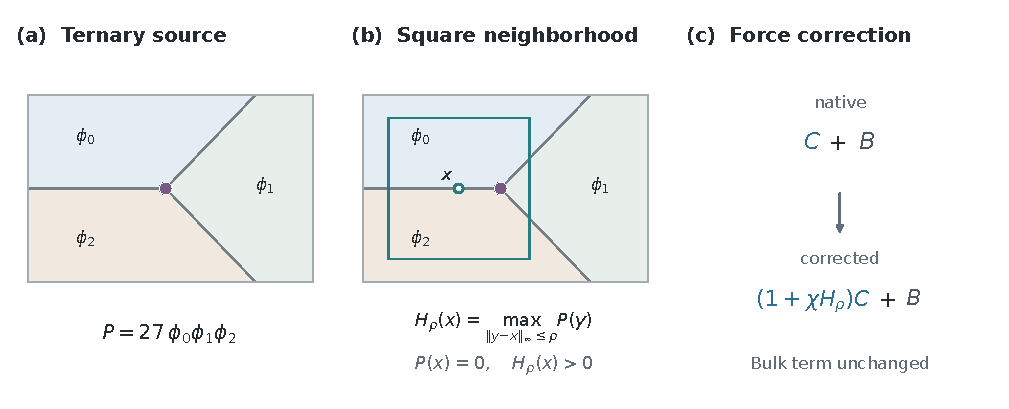
\includegraphics[width=0.96\linewidth]{method_schematic.pdf}
 \caption{Illustrative, not simulation-derived or to scale. (a) The source signal is $P=27\phi_0\phi_1\phi_2$. (b) The thin teal square is the width-$2\rho$ sampling region $\|y-x\|_\infty\leq\rho$, centered at binary receiver $x$ and containing the source: $P(x)=0$ but $H_\rho(x)>0$ (whole correction, $S=0$). (c) $(1+\chi H_\rho)$ weights capillary $C$ only; bulk $B$ is unchanged. No core angle is measured or implied.}
 \label{fig:method_schematic}
\end{figure}

A globally binary field has $P\equiv0$ and hence $H_\rho\equiv0$: the binary calibration problem is unchanged. A binary node near a junction can nevertheless receive a nonzero halo from neighboring ternary support. Source localization and output localization are therefore different. The multiplier satisfies $1\leq m\leq1+\chi$, but that bound is not a stability or accuracy guarantee.

Equation~\eqref{eq:corrected} changes the relative capillary and bulk forces. At a forced balance $\mathbf C+\mathbf B=0$, the corrected force becomes $(1-m)\mathbf B$, which need not vanish. The correction is consequently distinct from a uniform mobility or time change and is assessed against sharp-interface observables.

\subsection{Local memory after neighborhood overlap}
The optional memory variant suppresses selected ternary sources after correction neighborhoods overlap. At controller evaluations, label the eight-connected components of $\{P>0\}$. Components are incident when their radius-$\rho$ square dilations intersect. All components incident to an overlap are marked for suppression. A current component inherits suppression if it touches the preceding suppressed support dilated by one grid cell. Inheritance is updated after every Euler step, while new overlap is checked only at the prescribed controller times.

The stored object is a spatial support mask, not a permanent label number. Suppression removes sources before maximum filtering in Eq.~\eqref{eq:halo}; a nearby unsuppressed component can still contribute. This is a discrete history rule rather than a physical material-lineage model. It requires exact absent-phase values. Positive tails would change support topology and need a separately qualified construction. The exact label-window algorithm is given in the Supplementary Material.

\section{Benchmark design and measurements}
Lengths are normalized by strip width $W$, and time by $W^2/(M_0\gamma_0)$. The normalized pair energies are $\gamma_{01}=\gamma_{02}=1$, $\gamma_{12}=q$. For negative drive parameter $p$, the entries $\Delta f_{01}=\Delta f_{02}=-p>0$ favor phase 0; the grain--grain bulk force is zero. The equilibrium opening angle is $2\arccos(q/2)$.

The translating-front case uses $q=\sqrt3$, $p=-50$ and a $W\times4W$ moving domain. Matched runs begin from a common developed field and cover a further time of $0.25$. A separate cold comparison includes each route's binary calibration and junction evolution. The interacting case uses $q=1.5$, $p=-30$ and a $W\times24W$ domain containing junction pairs with nominal separations $7W$ and $10W$. Its comparison horizon is $0.12$. Outer boundaries have zero normal gradients.

For the cold controlled comparisons, a separate binary planar calculation fixes each recipe's clock factor
\begin{equation}
 a=V_{\rm target}/V_{\rm planar},\qquad t=s/a ,
 \label{eq:clock}
\end{equation}
where $s$ is raw solver time. This is the time coordinate corresponding to a uniform factor $a$ on the whole right-hand side. It is used for observation and controller scheduling, and is not fitted to junction outputs. Calibration is repeated if the stencil, grid, width or raw timestep changes. The original matched developed-front comparison retains the common nominal solver clock.

Migration speeds are fitted to interface-position and phase-area histories in settled windows. The translating-front shape is reconstructed at the same 92 physical transverse positions, interpolated before maximum alignment. Its RMS error is
\begin{equation}
 e_{\RMS}=\left[\frac1{92}\sum_{\ell=1}^{92}
 (\widehat y_h(x_\ell)-\widehat y_\star(x_\ell))^2\right]^{1/2}.
 \label{eq:rms}
\end{equation}
Alignment removes translation; this is not absolute-position error.

For grain consumption, marching-squares boundaries are compared in physical coordinates using symmetric Hausdorff distance
\begin{equation}
 \HH(\Gamma_h,\Gamma_\star)=
 \max\left\{\sup_{\mathbf x\in\Gamma_h}\inf_{\mathbf y\in\Gamma_\star}|\mathbf x-\mathbf y|,
 \sup_{\mathbf y\in\Gamma_\star}\inf_{\mathbf x\in\Gamma_h}|\mathbf x-\mathbf y|\right\}.
 \label{eq:hausdorff}
\end{equation}
Segment sampling supplies a distance bracket; it does not enclose continuum-model error. Disappearance time $T_{99}$ is bracketed when reconstructed grain area first falls to 1\% of its initial sharp-reference area. A boundary absent before its reference disappears is recorded as an empty-boundary outcome, never as zero error.

The operational accuracy targets are 5\% speed error and $0.05W$ shape error. They are study choices, not universal criteria. Settling uses early/late speed fits and aligned-profile changes; fraction bounds and the unit-sum constraint are checked separately. Numerical settings, schedules and reconstruction details are supplied in the Supplementary Material.

\section{Results}
\subsection{Matched correction of a developed driven front}
At $\eta=0.1W$, $h=0.005W$ and $\Dt_{\rm raw}=10^{-7}$, the native and corrected calculations share the physical matrices, stencil, projection, initial field and relative horizon. Their sole force-law difference is Eq.~\eqref{eq:corrected}. Migration-speed error falls from 16.014\% to 0.452\%, and terminal aligned RMS error from $0.105147W$ to $0.006016W$ (Fig.~\ref{fig:n20}). These are approximately 97.2\% and 94.3\% error reductions within this matched comparison.

The shape improvement extends over the profile and does not result from fitting its translation speed: both reconstructed shapes receive the same alignment operation. Both routes meet the retained settling and invariant criteria. Because they start from a common developed field, this test isolates the evolution correction but does not establish cold-start performance or supply its initialization for free in an end-to-end cost comparison.

\begin{figure}[tbp]
 \centering
 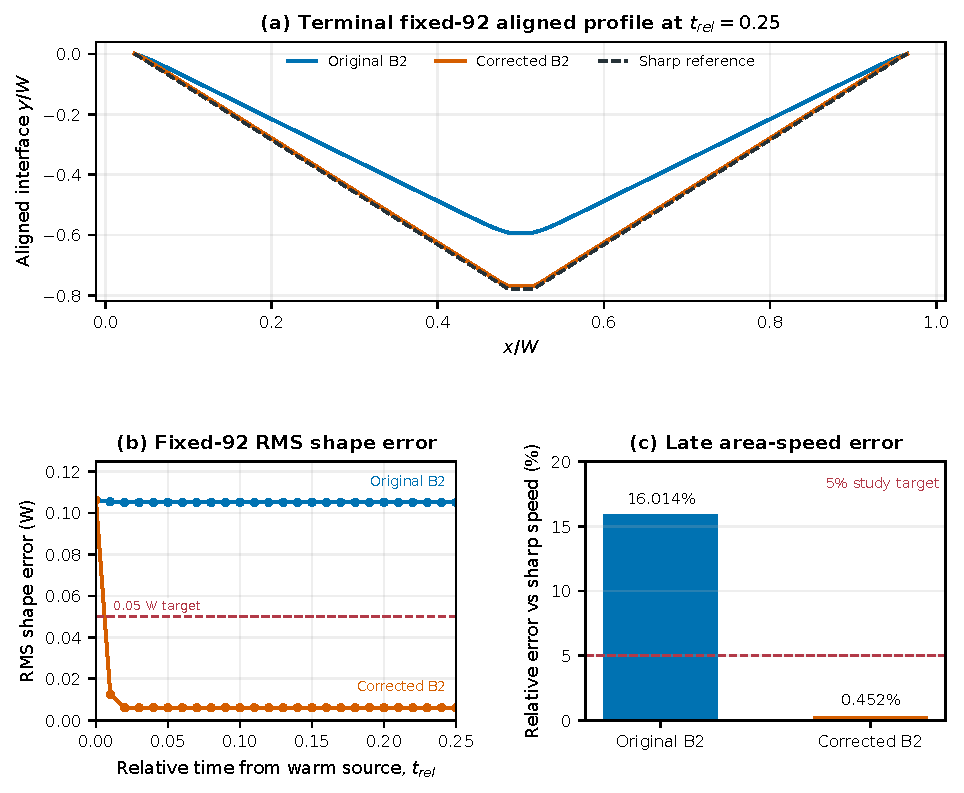
\includegraphics[width=\linewidth]{fig01_n20_matched.pdf}
 \caption{Matched translating-front comparison. Terminal profiles are maximum-aligned, and the dashed curve in panel (a) is the retained sharp reference. The shape history uses the fixed 92-point RMS definition. Time is elapsed time from the common developed state. The speed comparison uses the same sharp target. Both routes use $\eta=0.1W$, $h=0.005W$ and $\Dt_{\rm raw}=10^{-7}$.}
 \label{fig:n20}
\end{figure}

\subsection{Cold starts and a thinner conventional calculation}
A separate comparison starts each route from its width-specific compact profile and includes binary calibration. The corrected recipe uses $\eta=0.1W$, $h=0.01W$ and $\Dt_{\rm raw}=4\times10^{-7}$. The thinner conventional recipe uses $\eta=0.02W$, $h=0.005W$ and $\Dt_{\rm raw}=1.25\times10^{-6}$. The corrected route gives terminal aligned RMS error $0.004087W$ and speed error 1.326\%, compared with $0.013686W$ and 4.596\% for the selected thinner route.

Recorded end-to-end wall times, including calibration, are approximately 1035 and 1047~s. This pair therefore demonstrates better accuracy at a similar observed cost despite the wider interface and coarser grid. It does not isolate an intrinsic multiplier speedup: width, grid and timestep differ, and the observations are single realizations rather than an optimized accuracy--cost frontier.

\subsection{Interacting junctions and local memory}
\label{sec:interactions}
The cold interacting-junction test compares native, whole-correction and local-memory routes at the same $\eta=0.08W$, $h=0.01W$, nine-point Laplacian, raw timestep $4\times10^{-7}$, clock factor and initial field. Figure~\ref{fig:h24} and Table~\ref{tab:h24} show the largest sampled absolute shape errors.

\begin{table}[pos=htbp,abovecap=10pt]
\caption{Matched cold interacting-junction comparison. Entries are maximum sampled Hausdorff errors divided by $W$, distinct from the aligned RMS metric of Fig.~\ref{fig:n20}.}
\label{tab:h24}
\centering
\begin{tabular}{lrr}
\toprule
Method & Short pair & Long pair\\
\midrule
Native B2, nine-point stencil & 0.10609 & 0.14075\\
Whole spatial correction & 0.02694 & 0.03058\\
Spatial correction with local memory & 0.01399 & 0.01814\\
\bottomrule
\end{tabular}
\end{table}

The whole correction brings all sampled shapes below $0.05W$. Local memory supplies a further reduction of approximately 48.1\% and 40.7\% in the two worst sampled errors, with identical disappearance-time brackets for the two corrected routes. Memory thus supplies additional shape margin rather than being necessary to meet the selected tolerance.

At doubled raw timestep $8\times10^{-7}$, separately completed whole and local calculations retain worst errors $0.02696W/0.03064W$ and $0.01404W/0.01820W$. Both meet speed, disappearance-time and sampled-shape targets. Recorded peak resident memory is approximately 459 and 912~MB, respectively. Wall times were measured in different execution contexts and do not isolate controller overhead.

Other controls limit the interpretation. At $\eta=0.12W$, persistent memory improves two postinteraction shape samples by approximately 39\% and 13\% relative to a cadence-reset variant, although both variants meet $0.05W$. In an asymmetric interaction, whole and local routes give worst errors $0.01586W$ and $0.01437W$; the local route costs more in that sequential comparison. These observations support a case-dependent history benefit, not a requirement for memory whenever junctions interact.

\begin{figure}[tbp]
 \centering
 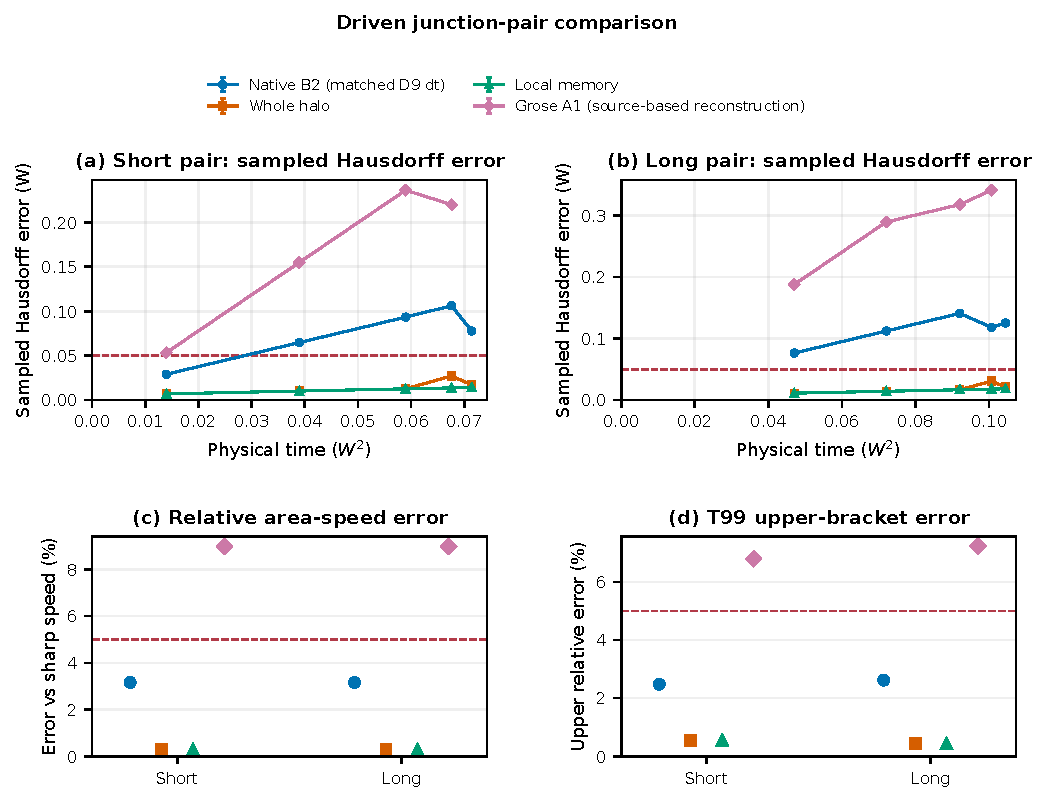
\includegraphics[width=\linewidth]{fig02_h24_routes_grose.pdf}
 \caption{Driven grain-consumption comparisons. The native, whole-correction and local-memory B2 routes share the cold initial field, width, grid, nine-point stencil and raw timestep. The Grose--Asimow reconstruction is a distinct source-based formulation at the same width and grid, with its own binary clock and numerical ingredients. Its selected recipe is compared, not the entire method's attainable performance. The fifth reconstructed-method shape observation for each pair has an empty boundary and therefore no finite ordinate.}
 \label{fig:h24}
\end{figure}

\subsection{A reconstructed high-driving-force method}
Grose--Asimow \citep{grose2022} is the closest conceptual comparator because it directly treats large driving forces at multiphase junctions. We reconstructed its force allocation, recursive transfer, finite-difference correction and grouped profile-restoration procedure. The operative pair equations are used where a printed segregation-sign expression conflicts with them. The numerical conventions needed for profile-anchor tracing and simultaneous events are documented in the Supplementary Material.

At the interacting-case width and grid, the declared amplification settings $A_\sigma=0$ and 1 do not meet the joint shape-and-kinetics targets. For the selected $A_\sigma=1$ half-step control, migration speed remains approximately 8.98\% above the sharp reference. Eight finite shape samples exceed $0.05W$, and two late boundaries are absent. Halving the timestep changes fitted speed by approximately 0.069\%, while shape discrepancies persist.

This compares specified independent implementations on a new driven unequal-energy interaction geometry. It is not a reproduction of the authors' executable or every published figure, nor an optimization of the free amplification parameter. The result supports an accuracy advantage over these reconstructed recipes on the present outputs. It does not establish failure of the published method in general or a speedup over its optimized implementation.

\subsection{Sensitivity to strength and radius}
\label{sec:robustness}
Four one-factor perturbations test the prescription $\chi=27$, $\rho=\eta$ in the developed-front case with $\eta=0.1W$ and $h=0.01W$. Strengths 20 and 34 are tested at radius ten cells; radii eight and twelve cells are tested at strength 27. The outcomes do not select a replacement baseline.

All four cases meet the retained speed, shape, settling and invariant criteria. Migration-speed errors range from approximately 1.07\% to 1.30\%, and terminal aligned RMS errors from $0.00366W$ to $0.00472W$ (Fig.~\ref{fig:robustness}). Thus the benefit is not restricted to one isolated parameter value in this case. These points do not define a continuous admissible region or an automatic parameter rule.

\begin{figure}[tbp]
 \centering
 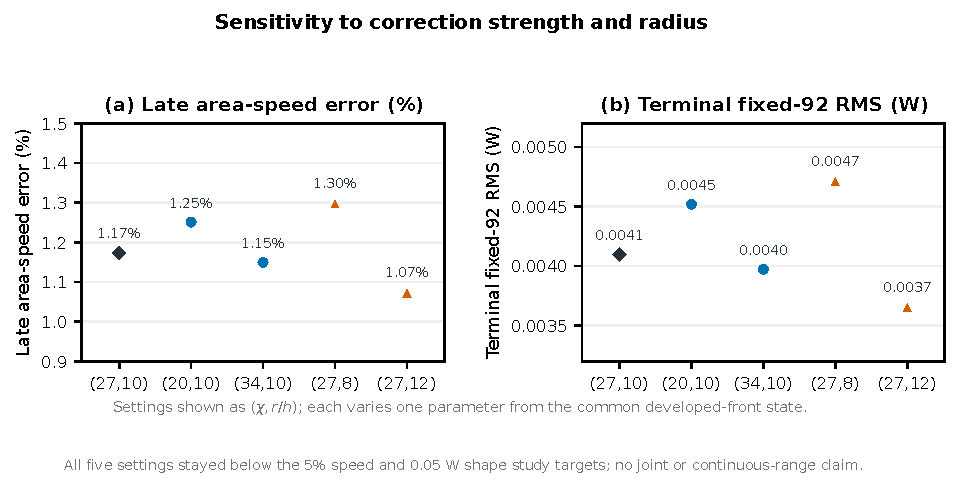
\includegraphics[width=\linewidth]{fig03_parameter_robustness.pdf}
 \caption{One-factor sensitivity around $\chi=27$ and $\rho/h=10$ in the developed-front benchmark. Strength and radius are perturbed separately. Points represent completed prescribed calculations, not a fitted parameter-response surface.}
 \label{fig:robustness}
\end{figure}

\subsection{Transfer to OpenPhase}
\label{sec:openphase}
We inserted the whole spatial correction into OpenPhase Academic \citep{tegeler2017}, using the pinned source revision specified in Ref.~\citep{openphase}. OpenPhase has its own local phase storage, pair assembly, driving-force merge and increment normalization. Only existing antisymmetric capillary increments are scaled, after native capillary calculation and before bulk-force merging. These operations are not replaced by our B2 kernel or Euclidean projector. The fixed prescription remains $\chi=27$, $\rho=\eta=0.08W$, giving eight cells at $h=0.01W$. The raw timestep remains $10^{-6}$.

Cold native and corrected trajectories share the initial field, boundaries, schedule, binary clock and $0.12$ horizon. Migration-speed error decreases from 25.532\% to 0.983\%. Short-pair $T_{99}$ error falls from a 15.736--16.031\% bracket to 0.787--1.084\%; the long-pair bracket falls from 17.226--17.430\% to 0.784--0.992\%.

Shape improvement is substantial but incomplete (Fig.~\ref{fig:openphase}). All five short-pair samples meet $0.05W$, with largest sampled error $0.04570W$. Four of five long-pair samples meet that target. At $t=0.10068814$, the remaining sample has error $0.05862W$ and sampling bracket $[0.05857W,0.05867W]$, entirely above the target. The next sample gives $0.04826W$. The fixed correction therefore improves this second implementation without refitting but does not remove every late shape discrepancy.

A fixed-grid, two-level timestep check repeats the same cold OpenPhase initial field and prescription at raw step $5\times10^{-7}$ to the same physical horizon, with a separately calibrated binary clock. The signed speed errors are $-25.595\%$ (native) and $-0.982\%$ (whole correction), close to $-25.532\%$ and $-0.983\%$ at $10^{-6}$. Corrected short- and long-pair $T_{99}$ errors remain within 5\% (0.787--1.085\% and 0.785--0.993\%); the corrected shape outcomes are again five of five short-pair passes and four of five long-pair passes. The late long-pair sample remains above $0.05W$ at $0.05859W$, including its sampling bracket. This is a two-level fixed-grid sensitivity check, not an asymptotic convergence study; detailed readouts are in Supplementary Table~S2.

Saved preinteraction fields also permit fixed-window fits of outer interface profiles away from the ternary diffuse core and correction support. In B2, the fitted two-arm included angle changes from 72.835--72.842$^\circ$ (native) to 60.093--60.094$^\circ$ (corrected), against a same-window sharp value of $60^\circ$. In OpenPhase, the corresponding descriptive upper/lower profile-corner angle changes from 63.918--63.925$^\circ$ to 82.251--82.480$^\circ$, against same-window sharp values of 82.819--82.997$^\circ$. These are outer-profile descriptors, not core selection angles. The native signed speed errors have opposite signs in the two implementations (+16.014\% in B2 and $-25.532\%$ in OpenPhase), so the geometric response does not establish a common positive-drag mechanism. Fit windows and definitions are given in Supplementary Table~S3.

\begin{figure}[tbp]
 \centering
 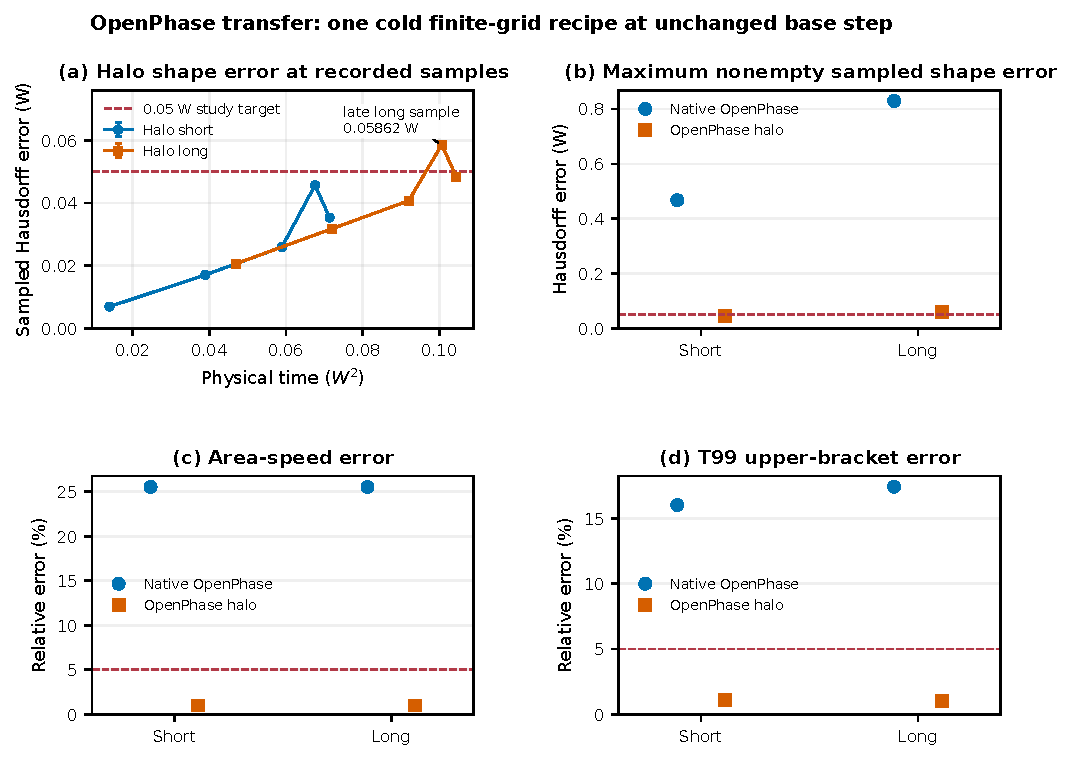
\includegraphics[width=\linewidth]{fig04_openphase_transfer.pdf}
 \caption{Fixed-prescription transfer to OpenPhase. Shape distances use actual saved physical times and the same sharp-reference construction. The long-pair sample above $0.05W$ is retained. Maxima in panel (b) include only nonempty boundaries; native empty-boundary observations are additional failures rather than zero distances. Passing migration-speed and disappearance-time targets does not imply accurate morphology at every sampled time.}
 \label{fig:openphase}
\end{figure}

\section{Discussion}
The demonstrated benefit is better junction shapes and kinetics at selected finite interface widths. The matched-front test separates this improvement from refinement or a changed clock. Interacting calculations show why whole-boundary shape matters in addition to preinteraction speed. The cold thinner-interface comparison supplies one useful accuracy--cost point, and the OpenPhase transfer shows that the prescription can retain a substantial benefit outside the original force assembly.

The multiplier acts over a neighborhood of ternary coexistence, including adjoining binary segments. It can therefore alter the relation between core motion and the surrounding interface. This motivates the construction but does not derive a selected junction geometry or identify a unique cause of every improvement. In particular, the multiplier scales curvature contributions as well as profile restoration. It is not equivalent to normal-only stabilization \citep{feyen2023}, and it does not generally preserve forced equilibria of the original model.

Local memory addresses a second issue: a correction useful for separated junction neighborhoods need not remain equally useful after those neighborhoods interact. Suppressing incident sources and retaining that decision can reduce postinteraction shape errors without globally switching off unrelated junctions. The whole correction already succeeds in the principal matched interaction case. Memory is consequently an optional refinement for additional shape margin, rather than a default requirement.

Conventional choices remain adequate in some regimes. Retained alternative-angle and asymmetric controls include cases where an economical native discretization performs well on the requested observables. The correction is not established as a universal replacement for refinement, mobility selection or existing high-drive models. Its useful setting is one in which finite-width junction error remains important and the chosen prescription has been checked against a relevant reference.

Three limitations matter for applying the method. First, strength and radius are empirical. The sampled perturbations and transfer reduce concern about an isolated fit but do not supply automatic parameter selection. Second, the demonstrations concern planar compact-support fields, common pair mobility and prescribed forcing. They do not establish performance for anisotropic surface stiffness, diffusion-coupled transformations, three-dimensional networks or smooth-tailed phase fields. Third, the evidence is finite-setting accuracy evidence. A retained profile/mesh comparison gives $0.002096W$ discrepancy against a $0.002W$ target and remains outside that target. The added OpenPhase check compares two timesteps on one grid and therefore provides sensitivity evidence, not a convergence rate. Width, grid and timestep are not independently taken to zero throughout the campaign, so the reported gain is not a continuum-convergence result.

The contribution relative to previous work is a distinct improvement on a defined task. The driven-junction benchmark \citep{hoffrogge2025}, force allocation and profile correction \citep{grose2022}, normal-profile stabilization \citep{feyen2023} and coarse-grid preconditioning \citep{sakane2026} address related parts of quantitative phase-field simulation. The spatial construction adds an implementable option, supported here by matched accuracy gains, interacting-boundary shapes and fixed-prescription OpenPhase transfer.

\section{Conclusions}
A neighborhood maximum of ternary coexistence localizes capillary amplification in compact-support multiphase-field calculations. At matched numerical settings it substantially improves the migration speed and aligned shape of a strongly driven unequal-energy junction. In cold interacting-junction calculations it reduces absolute whole-boundary shape error, while optional component memory supplies additional case-dependent accuracy after neighborhood overlap.

The same whole-correction prescription improves motion and disappearance timing in OpenPhase without refitting strength or relative radius. A remaining late shape error shows why speed and event timing cannot alone establish morphological accuracy. The method offers a demonstrated correction for the tested finite-width driven-junction regimes, with a simple whole-neighborhood form and an optional history-dependent refinement.

\section*{Data and code availability}
Numerical data underlying the figures, figure-generation code and recipe documentation are included in the accompanying source archive. A versioned Zenodo deposit of the study's reproducibility package is planned; its permanent DOI will be added before submission. OpenPhase is publicly available \citep{openphase}; the source revision and insertion point used here are specified in Section~\ref{sec:openphase} and the Supplementary Material.

\section*{Supplementary material}
The Supplementary Material provides force-channel construction, stencils, the component-memory algorithm, clock calibration, benchmark settings and reconstruction conventions, including the scope of the published-method comparison.

\section*{Declaration of generative AI and AI-assisted technologies}
ChatGPT was used to assist with this work, including coding and debugging. The author reviewed and edited the AI-assisted material and takes full responsibility for the content of this article.

\section*{Acknowledgments}
The author acknowledges the Kuwait Institute for Scientific Research (KISR) for institutional affiliation and general research support.

{\raggedright
\bibliographystyle{elsarticle-num}
\bibliography{references}
}
\end{document}
